\documentclass{article}
\usepackage[utf8]{inputenc}

\usepackage{enumitem}
\usepackage{graphicx}
\usepackage{subcaption}
\usepackage{float}
\usepackage{amsmath}
\usepackage{amssymb}
\usepackage{setspace}
\usepackage{xfrac}
\usepackage{indentfirst}
\usepackage{tikz}
\usepackage{hyperref}
\usetikzlibrary{positioning, fit, calc, arrows,shapes.gates.logic.US,shapes.gates.logic.IEC,}
\usepackage[siunitx, RPvoltages]{circuitikz}

\usepackage{enumitem}

\title{ECE350 Final Review - Cramming Carnival Solutions}
\author{Author: Members of HKN}
\date{}
\newcommand{\dd}[1]{\mathrm{d}#1}

\usepackage[makeroom]{cancel}
\usepackage[letterpaper, portrait, margin=1in]{geometry}
\usepackage{graphicx}

\pagenumbering{arabic}

\begin{document}

\maketitle

\section{Fiber Optics}
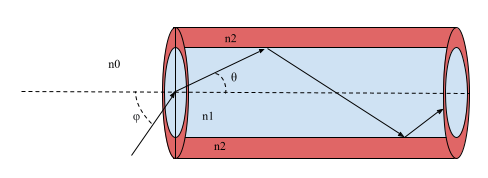
\includegraphics{figures/Optical Fiber Diagram.png}
The diagram above shows an Optical Fiber that is hit with a beam of light that enters the core(blue) of the fiber optic cable. The refractive index for the core $n_{1}=1.66$, the refractive index for the cladding(red) $n_{2}=1.63$, and the refractive index for air $n_{0}=1$. The wavelength of the light shown is $1200 nm$.

\subsection{Solution:}
\begin{enumerate}[label=(\alph*)]
    \item \textbf{Find the maximum value of $\varphi$ such that the wave is contained within the core(i.e., there is Total Internal Reflection when the wave in the core hits the cladding).}
    
    The first step to solving this problem is to find the critical angle between the core and the cladding. 
    $$\theta_{c} = \sin^{-1}(\frac{n_{1}}{n_{2}})$$
    $$\theta_{c} = 79.09^{\circ}$$
    Using $\theta_{c}$ we can find $\theta$ with the knowledge that both angles are part of the same right triangle so 
    $$\theta = 90 - \theta_{c}$$
    which means 
    $$\theta \le 10.91$$
    We can now find the maximum value of $\varphi$ using Snell's law with our answer for theta
    $$n_{0}\sin(\varphi) = n_{1}\sin(\theta)$$
    $$\sin(\varphi) \le \frac{n_{1}}{n_{0}}\sin(\theta)$$
    $$\varphi = \sin^{-1}(1.66\sin(10.91))$$
    $$\boxed{\varphi \le 18.31^{\circ}}$$
    
    \item \textbf{For the following questions, the Optical Fiber is now given a coating around the cladding with a refractive index $n_{3}=1.7$, $\varphi=10^{\circ}$, and we are operating in TE mode.}
    \begin{enumerate}[label=(\roman*)]
        \item \textbf{Find the angle of incidence of the wave in the core onto the cladding.}

    We can find the angle of incidence onto the cladding by reversing the process used in part a, starting by finding $\theta$ with Snell's law.
    $$n_{0}\sin(\varphi) = n_{1}\sin(\theta)$$
    $$\sin(10) = 1.66\sin(\theta)$$
    $$\theta = 6.005^{\circ}$$
    With the understanding that $\theta$ and the incident angle $\theta_{i}$ are both angles in a right triangle, we can do simple subtraction to find the incident angle
    $$\theta_{i} = 90 - \theta$$
    $$\boxed{\theta_{i} = 84^{\circ}}$$
        \item \textbf{ What should the width d of the cladding be such that the transmittance is .0001 at the coating that surrounds the cladding?}
        
    Our first step in finding the width of the cladding is to find $\Gamma_{21}$ using our transmittance.
    
    $$1 - \lvert\Gamma_{21}\rvert^{2} = .0001$$
    $$\Gamma_{21} = \sqrt{.9999}$$
    $$\Gamma_{21} = .9995$$
    
    Now that we have found $\Gamma_{21}$ we can find $Z(d)$, but first we need to find the impedance of the mediums which can be found using the refractive indexes as shown below.
    
    $$\eta_{3} = \frac{\eta_{0}}{n_{3}} \qquad\eta_{2} = \frac{\eta_{0}}{n_{2}} \qquad\eta_{2} = \frac{\eta_{0}}{n_{1}}$$
    
    We can solve for $Z(d)$ with the equation below.
    
    $$\Gamma_{21} = \frac{Z(d)-\frac{\eta_{1}}{\cos(\theta_{i})}}{Z(d)+\frac{\eta_{1}}{\cos(\theta_{i})}} $$

    $$.9995 = \frac{Z(d)-23.8}{Z(d)+23.8} $$

    $$Z(d)*(1-.9995) = 23.8*(1+.9995)$$

    $$Z(d) = 951,976$$

    Now that we have $Z(d)$, we can solve for d using the equation below

    $$Z(d) = \frac{\eta_{1}}{\cos(\theta_{i})}*\frac{1+\Gamma_{32}e^{-j2k_{2}\cos(\theta_{2})d}}{1-\Gamma_{32}e^{-j2k_{2}\cos(\theta_{2})d}} $$

    Before we can solve the equation we need to find a couple of values namely $\Gamma_{32}$, which is given by the equation below

    $$\Gamma_{32} = \frac{\eta_{3}-\eta_{2}}{\eta_{3}+\eta_{2}}$$
    $$\Gamma_{32} = \frac{\frac{1}{1.7}-\frac{1}{1.63}}{\frac{1}{1.7}+\frac{1}{1.63}}$$
    $$\Gamma_{32} = -.21$$
    
    We will start by solving for $a$ where $a = e^{-j2k_{2}\cos(\theta_{2})d}$ so we can focus on solving the equation before the exponential.

    $$Z(d) = \frac{\eta_{1}}{\cos(\theta_{i})}*\frac{1+\Gamma_{32}a}{1-\Gamma_{32}a} $$
    $$951976 = \frac{120\pi}{1.66*\cos(84^{\circ})}*\frac{1-.21a}{1+.21a}$$
    $$a = 47.4$$

    Now we can solve for $d$ using $a$ but first we'll need to find $\cos(\theta_{2})$ and $k_{2}$. To find $\cos(\theta_{2})$ we'll need to use Snell's law and the trigonometric identity $\sin^{2}(\theta) + \cos^{2}(\theta) = 1$.
    $$n_{1}\sin{\theta_{i}} = n_{2}\sin(\theta_{2})$$
    $$\sin(\theta_{2}) = \frac{1.66}{1.63}\sin(84^{\circ})$$
    $$\sin(\theta_{2}) = 1.013$$
    Now for the trig identity
    $$\sin^{2}(\theta_{2}) + \cos^{2}(\theta_{2}) = 1$$
    $$(1.013)^2 + \cos^{2}(\theta_{2}) = 1$$
    $$\cos(\theta_{2}) = \sqrt{1-1.026}$$
    $$\cos(\theta_{2}) = .162j $$
    $k_{2}$ can be found using the wavelength of the wave and the reflection coefficient as seen in the equation below.
    $$k_{2} = \frac{2\pi}{\lambda}n_{2}$$
    $$k_{2} = 8.53*10^{6}\; m^{-1}$$
    Now that we have all our parts we can find $d$
    $$a = e^{-j2\cos(\theta_{2})k_{2}d}$$
    $$47.4 = e^{2*d*.161*8.53*10^{6}}$$
    $$\frac{\ln(47.4)}{2*.161*8.53*10^6} = d$$
    $$\boxed{d = 1.4\; mm}$$
    
    
        \item \textbf{What is the angle of incidence of the wave transmitted through the coating?}

    The angle of incidence can be found using Snell's law between the first in third medium so,
    $$n_{1}\sin(\theta_{i}) = n_3\sin{\theta_{3}}$$
    $$\theta_{3} = \sin^{-1}(\frac{1.66}{1.7}\sin(84^{\circ}))$$
    $$\boxed{\theta_{3} = 76.2^{\circ}}$$
    \end{enumerate}
\end{enumerate}

\section{Waveguide Warm Up}
A parallel plate waveguide is filled with a dielectric with $\varepsilon=16*\varepsilon_{o}$. What is the spacing $a$, such that $5.5$ GHz is equal to $90\%$ of the $TE_{3}$ mode cutoff frequency?

\subsection{Solution:}

$$f_{c} = \frac{m*v}{2*a}$$
$$5.5*10^{9} = .9*(\frac{3*\frac{c}{4}}{2*a})$$
$$a = \frac{.9*9*10^{8}}{8*5.5*10^{9}}$$
$$\boxed{a = 18.4\; mm}$$

\section{Finding modes}
A given parallel plate waveguide contains an air-filled region with a plate separation $a = 10$ cm. Find the propagating $TE_{m}$ modes for a frequency of 5.5 GHz, and for each mode determine $f_{c}$, $\lambda_{g}$, and $\theta$.

\subsection{Solution:}

Start by finding the cutoff frequency in terms of the mode:

$$f_{c} = \frac{mc}{2a}$$
$$f_{c} = 1.5*10^{9}*m$$

From here we can increase m till the cutoff frequency is greater than our 5.5 GHz frequency. Doing so gives the active modes below and their respective cutoff frequencies.

$$\boxed{m=1\;f_{c}=1.5*10^{9}\;hz \qquad m=2\;f_{c}=3*10^{9}\;hz \qquad m=3\;f_{c}=4.5*10^{9}\;hz}$$

To find the guided wavelengths we'll need to use the equation below.

$$\lambda_{g} = \frac{2\pi}{k_{z}}$$
$$\lambda_{g} = \frac{2\pi}{\frac{\omega}{c}\sqrt{1-\frac{f_{c}^{2}}{f^{2}}}}$$
$$\lambda_{g} = \frac{c}{f\sqrt{1-\frac{f_{c}^{2}}{f^{2}}}}$$

Now using the cutoff frequencies from above we can find the guided wavelength for each mode.
$$\boxed{m=1\;\lambda_{g}=.057\;m \qquad m=2\;\lambda_{g}=.065\;m \qquad m=3\;\lambda_{g}=.095\;m}$$

The reflection angle $\theta$ can be found using the equation below.
$$\cos(\theta) = \frac{f_{c}}{f}$$
$$\boxed{m=1\;\theta=74.2^{\circ} \qquad m=2\;\theta=56.9^{\circ} \qquad m=3\;\theta = 35.1^{\circ}}$$

\section{Guided Waveguides}
We have a parallel plate waveguide that is filled with a dielectric with $\varepsilon=4*\varepsilon_{o}$. A signal frequency of 280 Mhz is propagating in the Waveguide. We have found that for the $TE_{2}$ mode the phase velocity is $v_{p} = 1.5*c$. Using this information we want to find the guided wavelength of $TM_{1}$ mode.

\subsection{Solution:}
\begin{enumerate}[label=(\alph*)]
    \item \textbf{Find the width, $a$, of the waveguide.}

    The first step is to use our phase velocity to find the cutoff frequency.

    $$v_{p} = \frac{v}{\sqrt{1-\frac{f_{c}^{2}}{f^{2}}}}$$
    $$1.5*c = \frac{\frac{c}{2}}{\sqrt{1-\frac{f_{c}^{2}}{(280*10^{6})^{2}}}}$$
    $$1-\frac{f_{c}^{2}}{(280*10^{6})^{2}} = \frac{1}{9}$$
    $$f_{c} = 280*10^{6}*\sqrt{\frac{8}{9}}$$
    $$f_{c} = 263*10^{6}$$

    Now that we have the cutoff frequency we can find $a$ knowing that the mode $m = 2$

    $$f_{c} = \frac{mv}{2a}$$
    $$263*10^{6} = \frac{2*\frac{c}{2}}{2*a}$$
    $$a = \frac{c}{2*263*10^{6}}$$
    $$\boxed{a = .57\; m}$$
    
    \item \textbf{Find the phase velocity, $v_{p}$, of the $TM_{1}$ mode.}

    Our first step is to find the cutoff frequency of the mode.

    $$f_{c} = \frac{mv}{2a}$$
    $$f_{c} = \frac{1*\frac{c}{2}}{2*.57}$$
    $$f_{c} = 131.6\; MHz$$

    Now we can use the cutoff frequency to find the phase velocity of $TM_{1}$

    $$v_{p} = \frac{v}{\sqrt{1-\frac{f_{c}^{2}}{f^{2}}}}$$
    $$v_{p} = \frac{\frac{c}{2}}{\sqrt{1-\frac{(131*10^{6})^{2}}{(280*10^{6})^{2}}}}$$
    $$\boxed{v_{p} = 1.7*10^{8}}$$
    
    \item \textbf{Find the guided wavelength, $\lambda_{g}$, of the $TM_{1}$ mode.}

    With the phase velocity of the mode we can very easily find the guided wavelength using the two equations below

    $$v_{p} = \frac{\omega}{k_{z}} \qquad \lambda_{g} = \frac{2\pi}{k_{z}}$$
    $$\lambda_{g} = \frac{2\pi}{\omega}v_{p}$$
    $$\lambda_{g} = \frac{v_{p}}{f}$$
    $$\boxed{\lambda_{g} = .607\; m}$$
\end{enumerate}

\newpage

\section{Disruptive Doppler}

Shomik is carrying a $\hat{z}$-polarized short dipole antenna, which is driven by an input current $i(t) = I_o cos(\omega t)$, where $\omega = 6 \cdot 10^9$ rad/s. Shomik is moving with the trajectory $(x, y, z) = (400 + 50t, 200 + 10t, t^2)$. Grant, moving with a trajectory of $(x, y, z) = (200 + 70t, 200 + 90t, t^2)$, is carrying another $\hat{z}$-polarized short dipole antenna which is displaying an open circuit voltage with a time-varying carrier phase $\Phi(t)$ in response to the field incident from Shomik's dipole. Assume free-space propagation for this problem.

\subsection{Solution:}

\begin{enumerate}[label=(\alph*)]
    \item Express the carrier phase $\Phi(t)$ explicitly in terms of $\omega$ and $t$. Hint: Shomik's dipole radiates a spherical wave of the form $cos(\omega t - kr)$. Hint 2: Be smart about your coordinate system choice.

    It is convenient to first lock Shomik at the origin and have Grant be the only one moving. We really want the distance between the two of them, so doing so preserves this distance but makes the math easier. Therefore, Shomik is now at the origin and Grant moves with trajectory $(x, y, z) = (200 + 70t, 200 + 90t, t^2) - (400 + 50t, 200 + 10t, t^2) = (-200 + 20t, 80t, 0)$.

    The radial distance from the origin can then be found using the Pythagorean theorem:

    $$r = \sqrt{(-200 + 20t)^2 + (80t)^2} = 20 \sqrt{100 - 20t + 17t^2}$$

    Finally, since we know $\omega$ and we're in free-space, we can easily find $k = \omega/c = 20$. Thus,

    $$\boxed{\Phi(t) = \omega t - kr = \omega t - 400 \sqrt{100 - 20t + 17t^2}}$$

    \vfill

    \item Given that $\omega' = \frac{\partial \Phi}{\partial t}$, what is the Doppler frequency shift $\omega' - \omega$ of Grant's open-circuit voltage at $t = 0$?

    We now take the derivative to find $\omega'$.

    $$\omega' = \omega - 400 \frac{34t - 20}{2\sqrt{100 - 20t + 17t^2}}$$

    We can then find the Doppler frequency shift:

    $$\omega' - \omega = - 400 \frac{34t - 20}{2\sqrt{100 - 20t + 17t^2}}$$

    Plugging in $t = 0$, we get

    $$\boxed{\omega' - \omega = 400 \text{rad/s}}$$

    This makes sense! At this time, Grant is moving towards Shomik, so he should see higher frequencies than what Shomik is outputting (draw out the trajectory!)

    \vfill

    \item What is the Doppler frequency shift $\omega' - \omega$ of Grant's open-circuit voltage at $t = 10$?

    Same Doppler frequency shift as above:

    $$\omega' - \omega = - 400 \frac{34t - 20}{2\sqrt{100 - 20t + 17t^2}}$$

    Plugging in $t = 10$, we get

    $$\boxed{\omega' - \omega = -400 \frac{320}{2 \sqrt{100 - 200 + 1700}} = -1600 \text{rad/s}}$$

    This makes sense! At this time, Grant is moving away from Shomik, so he should see lower frequencies than what Shomik is outputting (draw out the trajectory!)

    \vfill

    \item Find the time-point(s) at which the Doppler frequency shift $\omega' - \omega$ is zero. What is the physical significance of these time-points? How many such time-points are there?

    Simply set the Doppler frequency shift to $0$ and solve for $t$. We find that this holds when $\boxed{t = \frac{20}{34}}$. At this exact time-point, Grant is switching from moving towards Shomik to moving away from Shomik, so he will actually see the exact frequency that Shomik is outputting.

    This is the only such time-point - Grant's trajectory is linear with respect to Shomik's, and this time-point is the closest approach that Grant will ever have to Shomik. 

    \vfill

    \item Qualitatively, what is the behavior of the Doppler frequency shift at the limits $t \longrightarrow \infty$ and $t \longrightarrow -\infty$ (i.e. constant? linear? quadratic?)? Name the approximation that can you use in these cases (you've seen it before in ECE350!).

    The numerator is linear with respect to $t$, and the denominator is linear with respect to $\sqrt{t^2}$ in the limit. Thus, the Doppler shift should converge onto some constant in these limits. This is verified by graphing on Desmos.

    This is the $\boxed{\text{paraxial}}$ approximation at work! Far enough away, it looks like Grant is just moving away from Shomik at a constant velocity, so the Doppler frequency shift converges to a constant. Cool!

    \vfill

    \item Are the calculations above relativistically correct?

    No! This uses non-relativistic Doppler shift formulae.
\end{enumerate}

\newpage

\section{Clingy Conductors}

\begin{center}
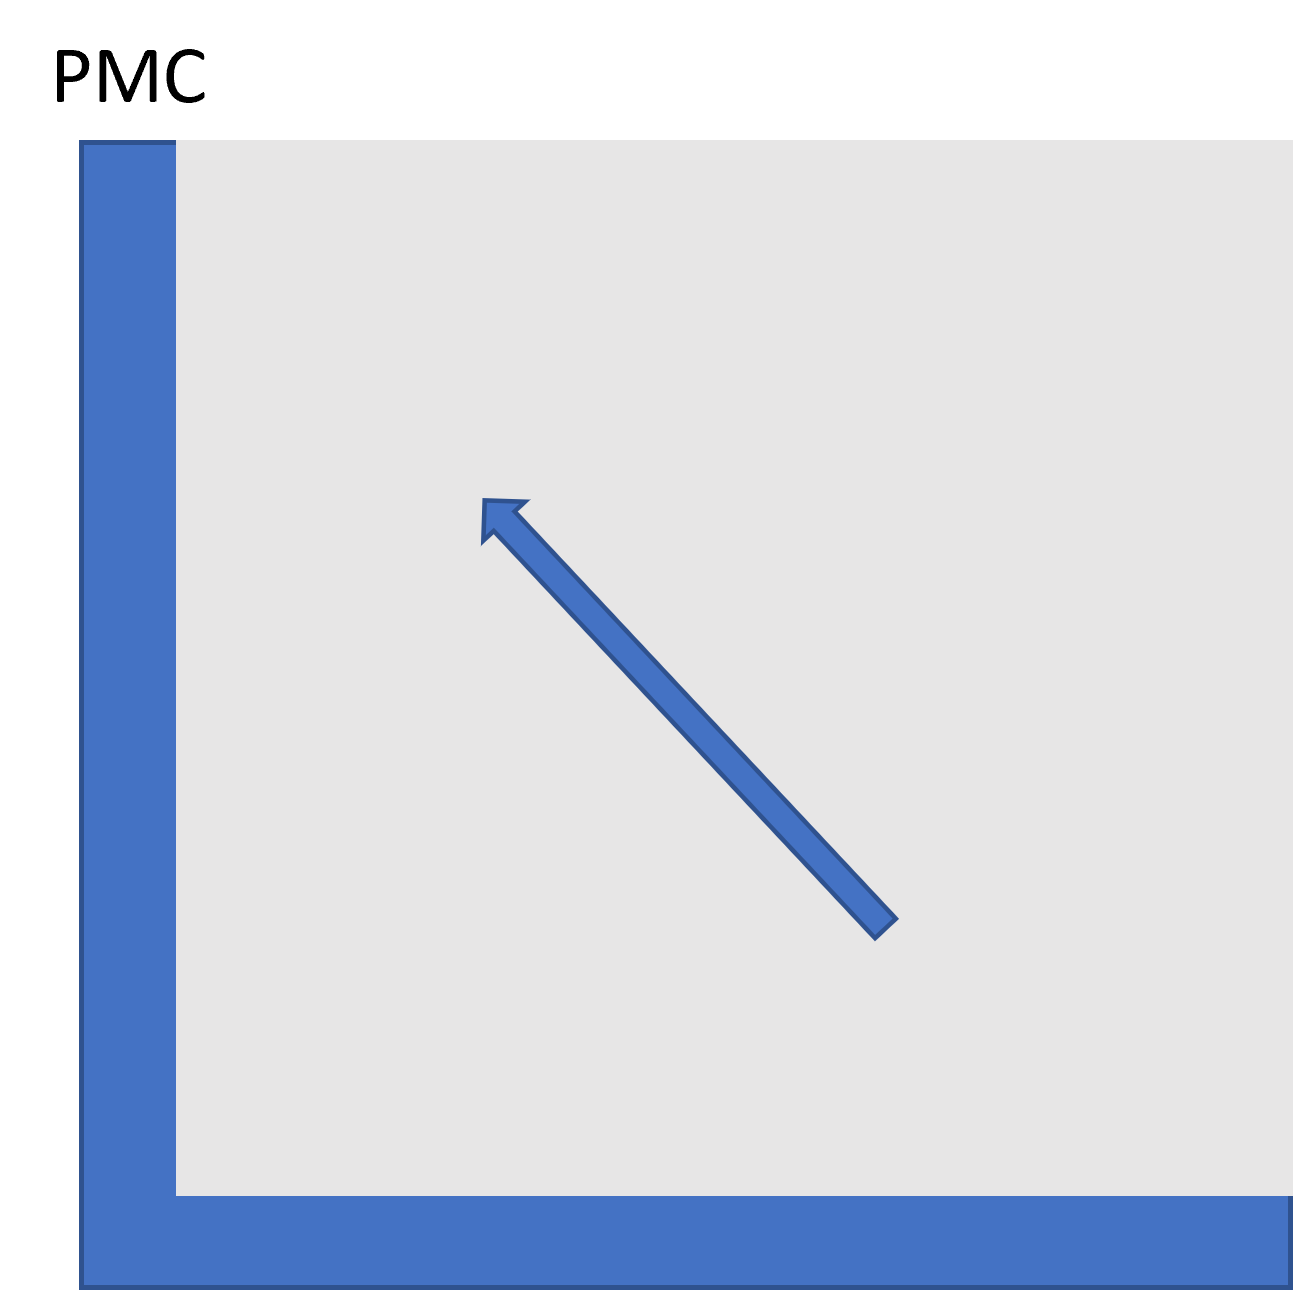
\includegraphics[width=0.5\textwidth]{figures/PMC Prompt.jpg}
\end{center}

Given the situation above, sketch the three image antennas resulting from the perfect \textbf{magnetic} conductor (PMC) (shown as the blue rectangles on the boundary) based on image theory. Recall that a PMC enforces the boundary condition that the tangential B field is zero (what does a PEC do instead?)

\subsection{Solution:}

The solution can be split into the following steps:

\begin{itemize}
    \item Split the dipole antenna into its component parts.
    \item Analyze the B-field resulting from each of the component parts. Recall that the B-field points in the $\phi$ direction.
    \item On the other side of the boundary, draw the image component that forces the B-field to be zero, as shown below:
    \begin{center}
    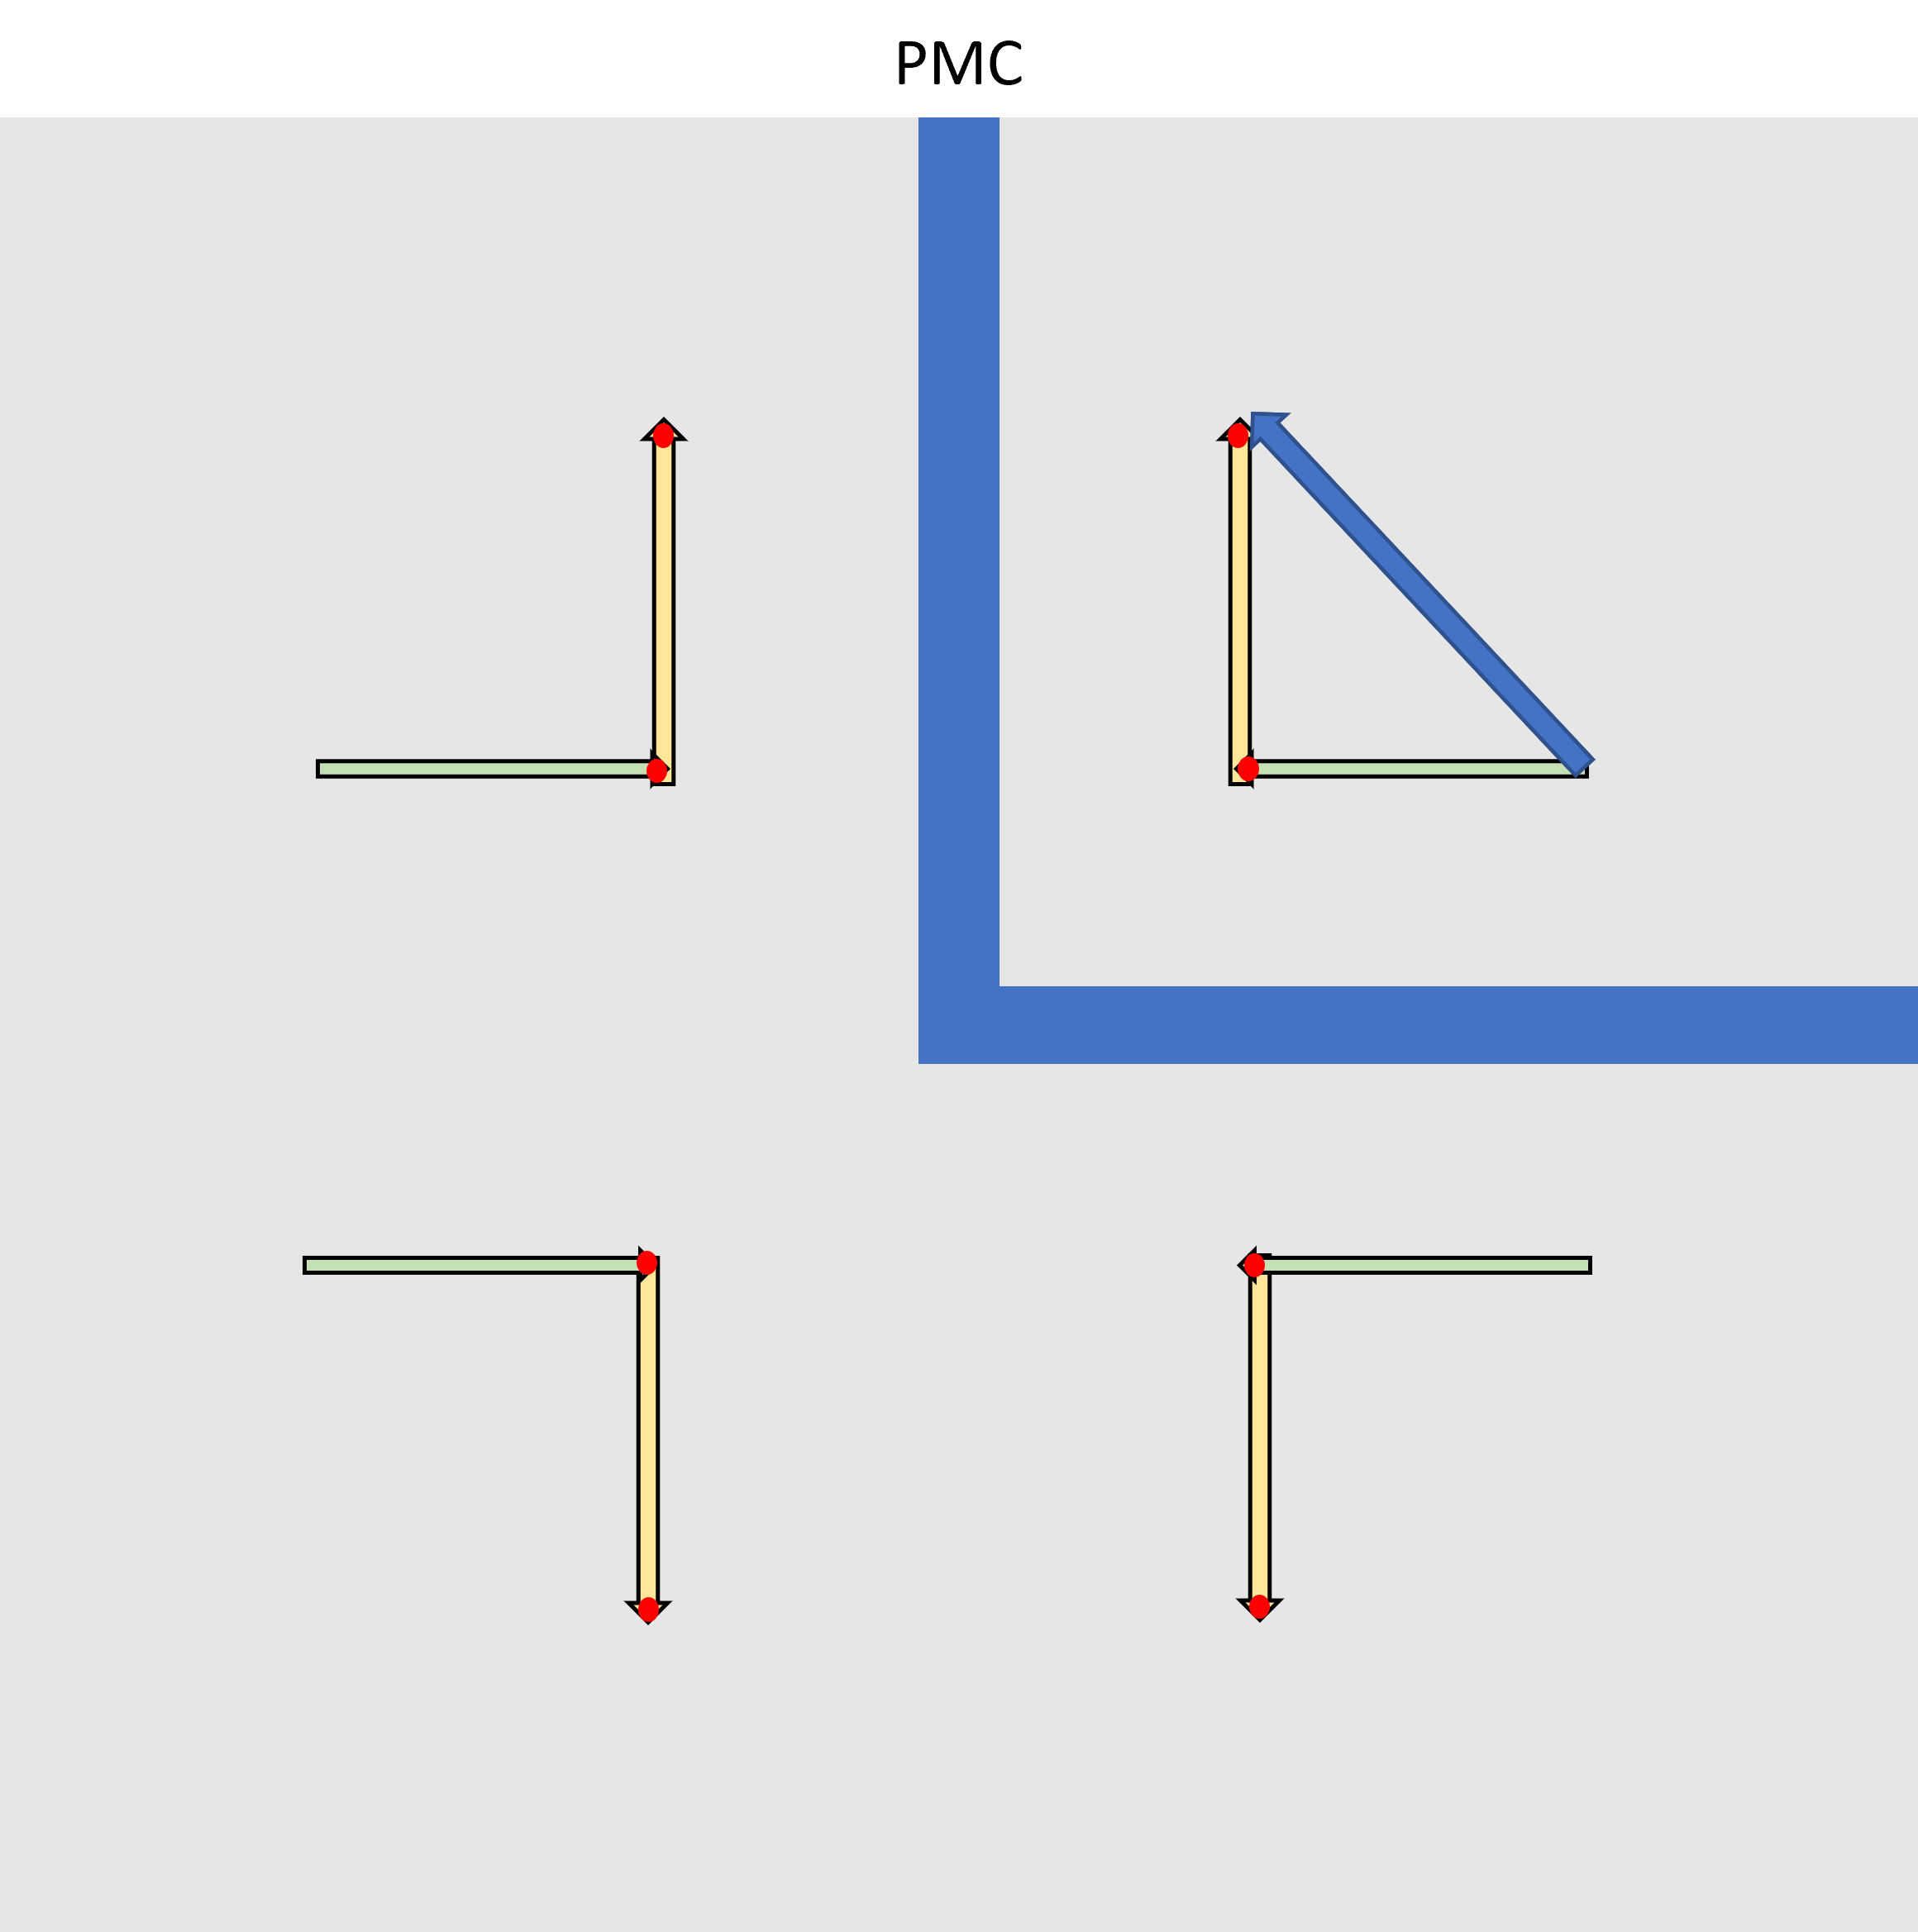
\includegraphics[width=0.5\textwidth]{figures/PMC Solution Initial.jpg}
    \end{center}
    \item Use basic vector addition to solve for the three image antennas, as shown below:
    \begin{center}
    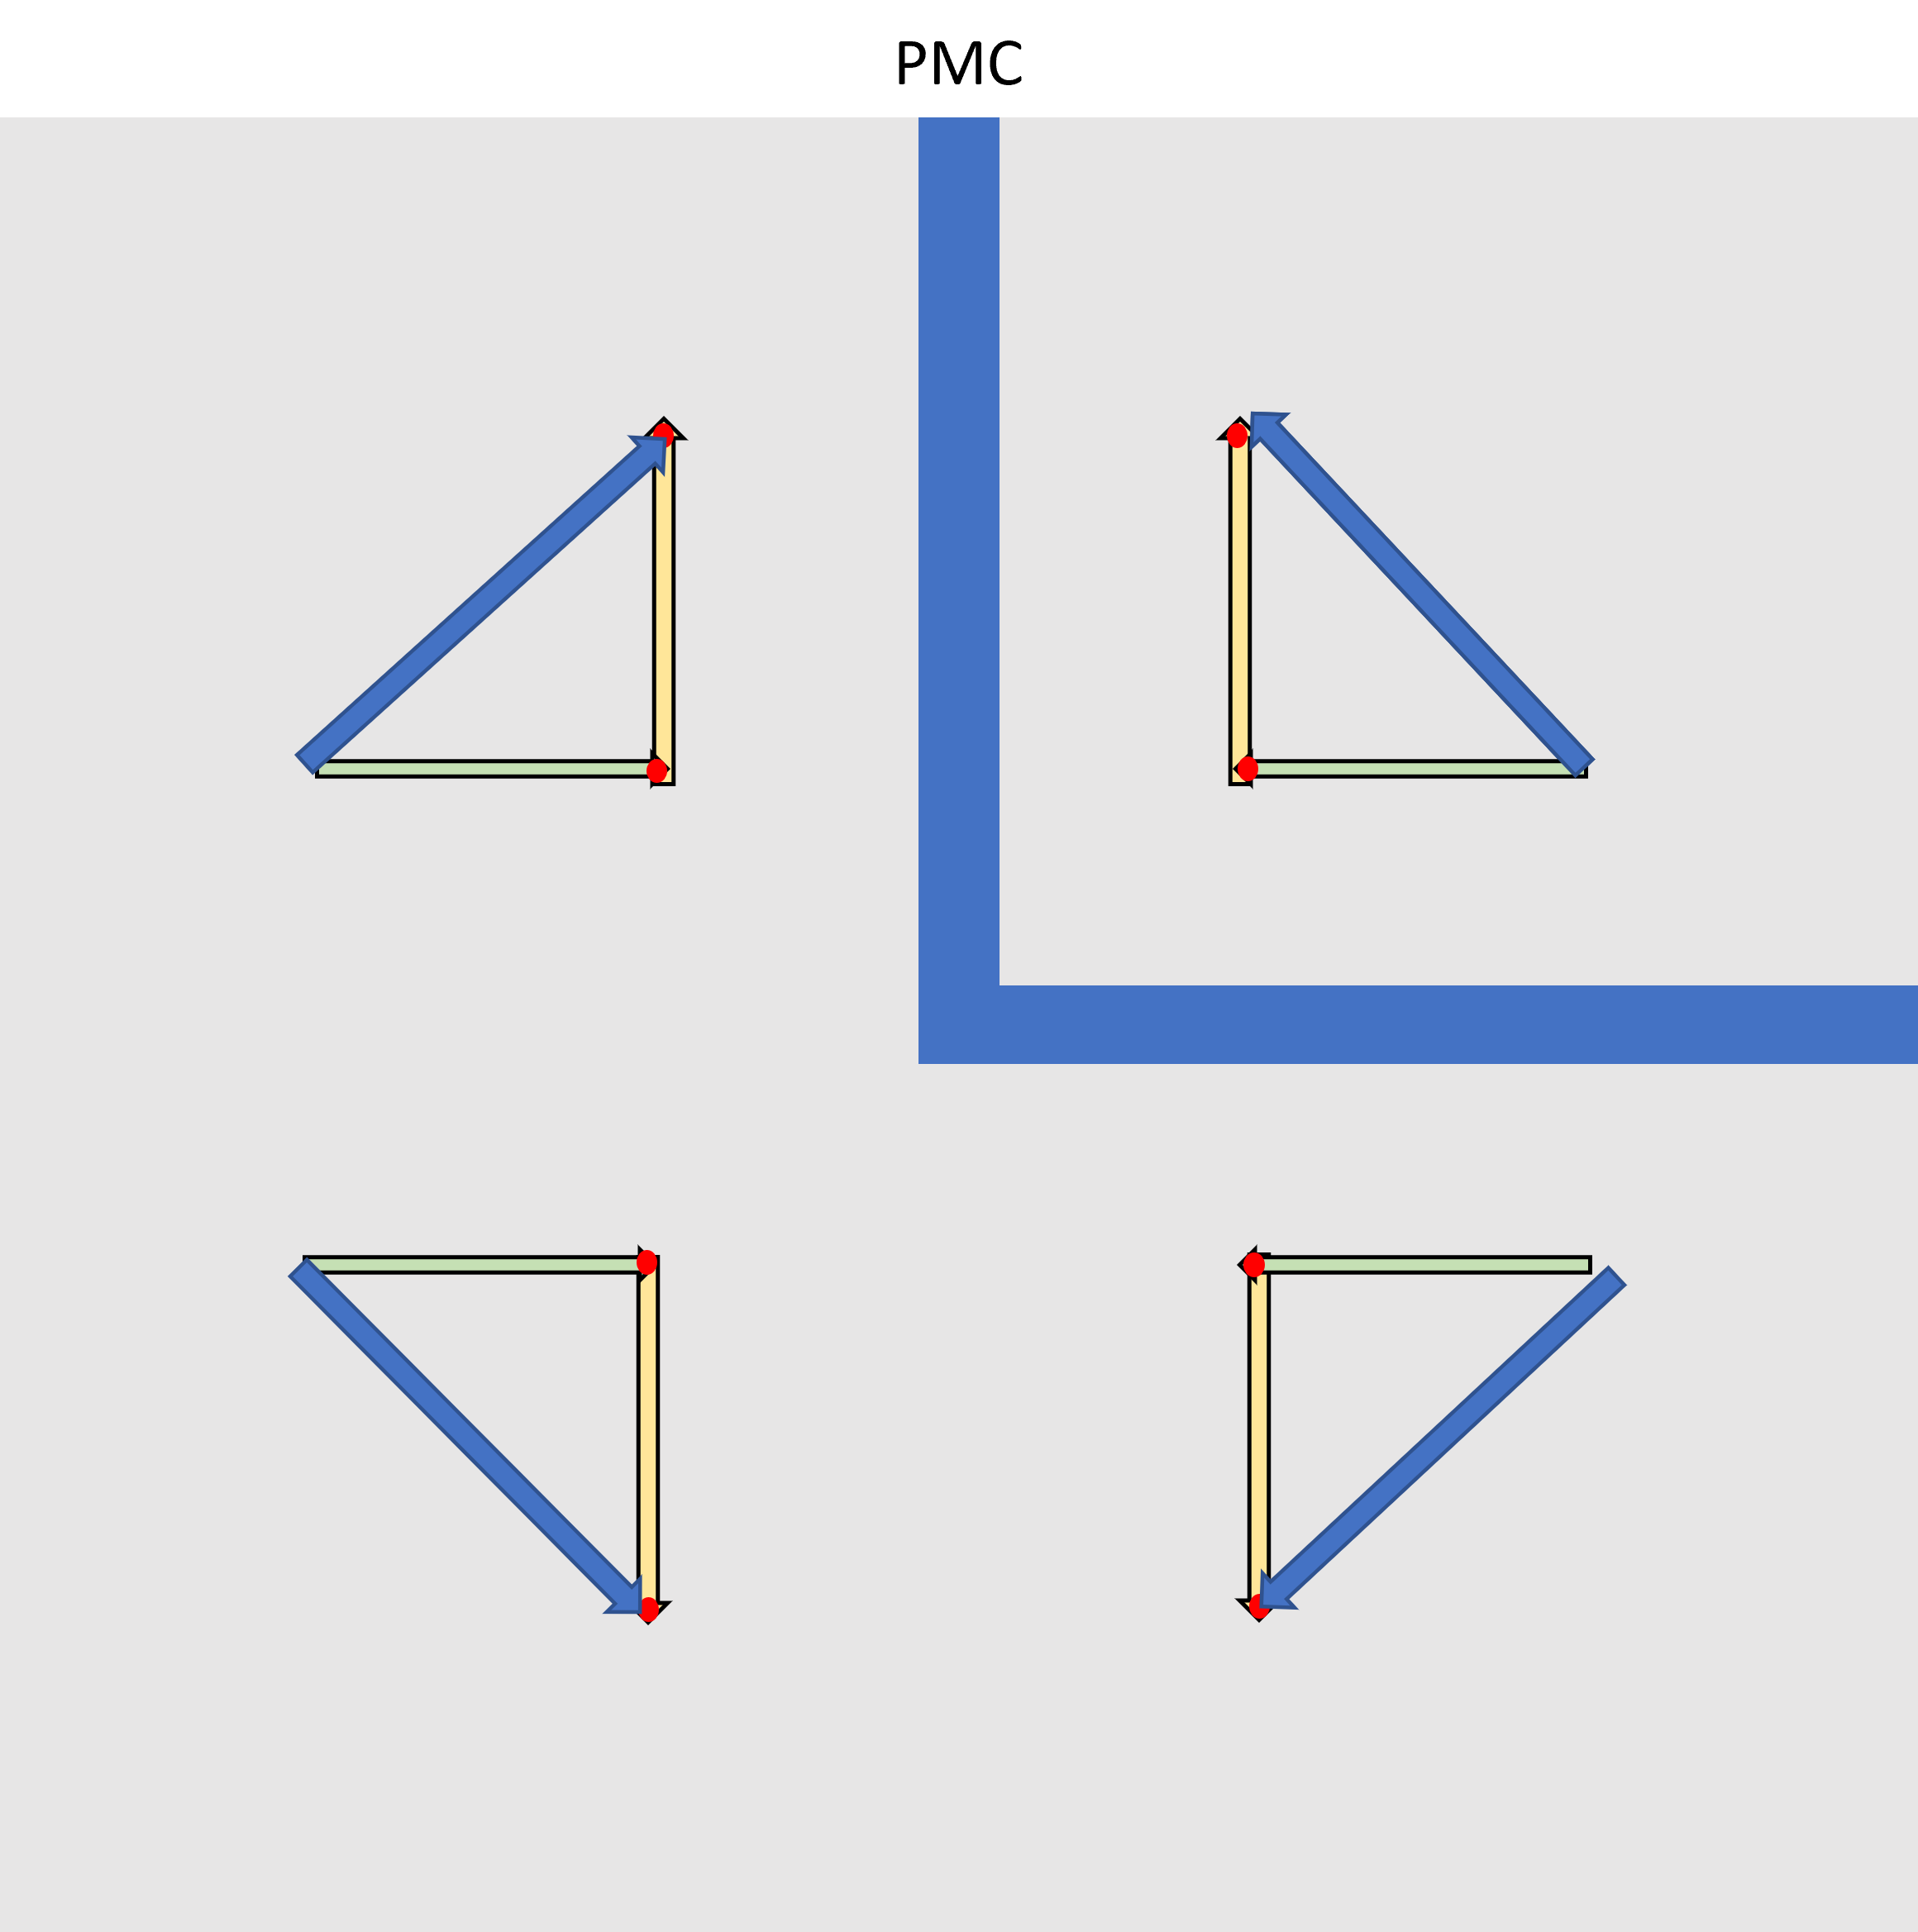
\includegraphics[width=0.5\textwidth]{figures/PMC Solution Final.jpg}
    \end{center}
\end{itemize}

\newpage

\section{Devious Duality}

\subsection{Solution:}

\begin{enumerate}[label=(\alph*)]
    \item A line of negative charges sit on the $x = 0$ axis. The charges have a density of $\lambda$ charges per meter. What is the electric field as a function of position given off by these charges? What is the magnetic field as a function of position given off by these charges?

    This is an ECE329 derivation that can be found online. The important thing is that there is an electric field, pointing into the wire, and no magnetic field.
    
    $$\boxed{\vec{E} = -\frac{\lambda}{2 \pi r \epsilon} \hat{r}}$$

    $$\boxed{\vec{B} = 0}$$

    \vfill
    
    \item You decide to now start travelling at $v = 0.5c$ in the $+\hat{x}$ direction. The charges now look like they are travelling at $0.5c$ in the $-\hat{x}$ direction. From your point of view, what is the electric field as a function of position given off by these charges? From your point of view, what is the magnetic field as a function of position given off by these charges?

    Moving charges constitute a current. The current can be found as $I = NqAv = \lambda q 0.5 c$ (note that $NA = \lambda$ in this case). This is also an ECE329 derivation that can be found online. The important thing is that there is no electric field, and there is a magnetic field circling around the current.

    $$\boxed{\vec{E} = 0}$$

    $$\boxed{\vec{B} = \frac{\mu_0 \lambda q 0.5 c}{2 \pi r} \hat{\phi}}$$

    \vfill
    
    \item Points of view do not affect what is really happening. So what is the underlying truth?

    The underlying truth is that electric and magnetic fields are fundamentally the same thing. This is why they are called electromagnetic fields. An electric field is simply a magnetic field from another point of view, and vice versa. Awesome.
\end{enumerate}

\newpage

\section{Rigid Reciprocity}

Let $\rho_1$ be a static charge distribution over free space with a corresponding potential distribution $\phi_1$, and $\rho_2$ be a static charge distribution over free space with a corresponding potential distribution $\rho_2$. 

\vspace{3mm}

Given Green's second identity on scalar functions:

\[
\int_U (\psi\nabla^2\varphi - \varphi\nabla^2\psi) dV = \oint_{\partial U}(\psi\nabla\varphi - \varphi\nabla\psi)\cdot dS
\]

prove Green's reciprocity theorem:

\[
\int \rho_1\phi_2 dV = \int \phi_2\rho_2 dV
\]

Note: The integral above is taken over $\textbf{all of free space}$. $\partial U$ represents the boundary of the set $U$.

\subsection{Solution:}

We first note that the charge distribution $\rho$ is related to the potential distribution $\phi$ via the following relation:

\[
\rho = -\epsilon\nabla^2 \phi
\]

We then rewrite the reciprocity theorem as follows, moving both integrals to the same side and applying the above relation:

\[
-\epsilon \int_S \phi_2\nabla^2\phi_1 - \phi_1\nabla^2\phi_2 dV = 0
\]

Applying Green's second scalar identity and dividing out the constant outside the integral:

\[
\oint_{\partial S} (\phi_1\nabla\phi_2 - \phi_2\nabla\phi_1)\cdot\textbf{S} = 0
\]

Since our set $S$ is the entire three-dimensional domain, we are then interested at the contour integral of this boundary at infinity; at infinity, $\nabla\phi_1$ and $\nabla\phi_2$, which are the electric field distributions for each respective potential function, both vanish at infinity, leading the integrand to be 0. 

As such, we see that 
\[
\int (\rho_1\phi_2 - \phi_2\rho_2 )dV = 0
\]

which proves the reciprocity theorem.

\subsubsection{Alternate Solution:} The Laplacian (denoted as $\mathcal{L}$) is a self-adjoint operator for the $L^2$ inner product on functions which vanish on the boundary. The $L^2$ inner product on real functions $f,g$  is defined as:

\[
\langle f, g\rangle = \int_U f(x) g(x) dx
\]

and since $\phi_1$ and $\phi_2$ both vanish on the boundary, we can say that:

\[
\langle \phi_1, \mathcal{L}\phi_2\rangle = \langle \mathcal{L} \phi_1, \phi_2\rangle
\]

We can expand the inner product and use $\rho = -\epsilon\nabla^2 \phi$ to directly get Green's reciprocity theorem.

\newpage

\section{Peanut Butter Dispute}

Shomik and Grant are very angry with each other (something about peanut butter apparently). Shomik gets on his spaceship and travels away from Earth at a velocity of $0.6c$.  At the same time, Grant gets on his spaceship and travels away from Earth in the opposite direction at a velocity of $0.6c$. In the meantime, Shomik and Grant continue to send curse words and insults to each other using a radio with a frequency of $\omega$. The signals they send take the form of $Acos(\omega t)$, where $A$ is some (varying) amplitude.

\subsection{Solution:}

\begin{enumerate}[label=(\alph*)]
    \item What is the frequency of the communication when detected from Earth?

    This is a simple plug and chug Doppler problem from lecture. We'll call our result $\omega_E$.

    $$\omega_E = \omega \sqrt{\frac{1 - 0.6}{1 + 0.6}} = \boxed{\frac{\omega}{2}}$$
    
    \item What is the frequency of Grant's communication as detected by Shomik?

    Grant's communication as detected on Earth is given by part (a). We can then use this value to figure out what Shomik detects, $\omega_S$.

    $$\omega_S = \omega_E \sqrt{\frac{1 - 0.6}{1 + 0.6}} = \boxed{\frac{\omega}{4}}$$
    
    \item Using the normal formulae for velocity addition, how fast is Grant moving away from Shomik? Is this correct?

    Grant is moving away from Earth at $0.6c$. Shomik is moving away from Earth at $0.6c$. Adding these up, Grant is moving away from Shomik at $\boxed{1.2c}$. No, this cannot be correct.
    
    \item Grant realizes that Shomik is not receiving his messages properly. What frequency must Grant use so that Shomik detects the frequency $\omega$?

    Simply invert part (b)'s final answer. Grant needs to use $\boxed{4\omega}$ instead.
\end{enumerate}

\newpage

\section{Time-Bender}

Shomik continues to send messages to Grant of the form $Acos(\omega t)$, which means that Grant receives them with the form $Acos(\omega' t - k'x) = Acos(\omega' t - k'vt) = Acos(\omega' \left(1 - \frac{v}{c} \right) t)$. Note that $\frac{\omega}{k} = c$ always in a vacuum, so if $\omega$ changes, then $k$ must also change. Also note the direction of our $x$-axis.

Grant now resorts to mocking Shomik instead. Grant then sends the exact same message back at the exact frequency that he received it at, aka $\omega'$. Shomik then receives his own message at frequency $\omega''$, enraging him further.

For this problem, assume that Grant is moving away from Shomik at velocity $v$. Be \textbf{extremely} careful about what point of view you are using. Really put yourself into Shomik's or Grant's shoes.

\subsection{Solution:}

\begin{enumerate}[label=(\alph*)]
    \item At what velocity is Shomik moving away from Grant? (Yes, this is trivial.)

    Also $\boxed{v}$. If Shomik thinks Grant is moving away at velocity $v$, then Grant must also think that Shomik is moving away at velocity $v$ by symmetry.
    
    \item What is $\omega'$, and $\omega''$? Express them as functions of $\omega$. Hint: Do problem 1 first.

    We note that $\omega'$ is the frequency that Grant is receiving his signals from Shomik. Thus, we simply report the general Doppler formula since we're only given $v$.

    $$\boxed{\omega' = \omega \sqrt{\frac{1 - \frac{v}{c}}{1 + \frac{v}{c}}}}$$

    Grant now sends out a wave with frequency $\omega'$. It will go through the exact same Doppler shift before it reaches Shomik. Therefore, we multiply it by the same factor again. This causes the square root to disappear.

    $$\boxed{\omega'' = \omega \frac{1 - \frac{v}{c}}{1 + \frac{v}{c}}}$$

    \item From Grant's point of view, what is the form of signal sent out by Grant? Write it out in the same format as provided (a cosinusoidal), although set $x = 0$ since Grant is always at the origin (from Grant's point of view). Leave you answer in terms of $\omega'$.

    From Grant's point of view, Grant's wave is sent out with frequency $\omega'$. Therefore, from Grant's point of view, this must've been the wave that was sent out by Grant.
    
    $$Acos(\omega' t + k'x) = \boxed{Acos(\omega' t)}$$
    
    \item From Shomik's point of view, what is the form of signal sent out by Grant? Write it out in the same format as provided (i.e. simplify your answer so that it does not use any version of $k$). Leave your answer in terms of $\omega''$.
    
    From Shomik's point of view, Grant's wave arrives with frequency $\omega''$. Therefore, from Shomik's point of view, this must've been the wave that was sent out by Grant. However, we also know that $\frac{\omega''}{k''} = c$. We start with

    $$Acos(\omega''t + k''x) = Acos(\omega''t + k''vt)$$
    
    $$\boxed{= Acos(\omega'' \left(1 + \frac{v}{c} \right) t)}$$

    Note that we require the $k''x$ term here because Shomik is actively moving away from Grant, who is the one actually generating the signal. Therefore, the phase of the wave is affected by the time that Shomik receives it, as well as how far he is away from Grant when he receives it. Also note that we use $+k''x$, since the wave travels from Grant to Shomik (in the $-\hat{x}$ direction).
    
    \item However, the signals in part (d) and part (e) must be the same signal - Grant and Shomik are just calling it different things. This is a fundamental postulate of physics: One's point of view \textbf{\textit{CANNOT}} affect the underlying truth (for if it did, this must be a single correct point of view, which feels very bad). Therefore, the solutions of (d) and (e) must be set equal to each other.

    But we know $\omega'' \neq \omega'$. What else must be changing as we switch from Shomik's point of view and Grant's point of view? Express the quantity from Grant's point of view in terms of the quantity from Shomik's point of view.

    The waves must be the same. The amplitude does its own thing on the outside and does not require modification. The speed of light must remain the same. The velocity must also be the same (by part (a)). Thus, if the frequencies are changing, $\boxed{\textbf{\textit{time}}}$ must be changing as we change point of views. This is an extremely counterintuitive result, but the conclusion is inescapable. This means that Grant, if he views Shomik's clock, will perceive that Shomik's clock is running differently than his own clock.
    
    We'll denote Grant's time as $t'$ and Shomik's time as $t$.

    We need $\omega't' = \omega''\left(1 + \frac{v}{c} \right)t$ in order for the two waves to match up exactly. Plugging in the results from part (b), we get

    $$t' \omega \sqrt{\frac{1 - \frac{v}{c}}{1 + \frac{v}{c}}} = t \omega \frac{1 - \frac{v}{c}}{1 + \frac{v}{c}}\left(1 + \frac{v}{c} \right)$$

    Now we simplify.

    $$t' = t \left(1 - \frac{v}{c} \right) \sqrt{\frac{1 + \frac{v}{c}}{1 - \frac{v}{c}}}$$

    $$t' = t \sqrt{\left(1 - \frac{v}{c}\right) \left(1 + \frac{v}{c} \right)}$$

    $$\boxed{t' = t\sqrt{1 - \frac{v^2}{c^2}}}$$

    Stop, and let this result sink in for a second. First, this doesn't depend on $\omega$, only of $v$, which means this is a completely general result that applies to any other situation. Secondly, two clocks simply moving at different, constant velocities, will become offset from each other.

    Note that since $v < c$ always, the factor on the right side is always less than $1$ and always positive. Therefore, $t' < t$: when Shomik believes that $t$ time has passed, Shomik will see that Grant's clock has progressed by $t'$ instead, which is less than $t$. This is called \textbf{time dilation}: time is dilating (or getting slower) as we look at someone speeding away from us.
\end{enumerate}

\newpage

\section{Space-Bender}

The above result has profound consequences. For this problem, assume that Grant is moving away from Shomik, from Shomik's point of view, at $v$.

\subsection{Solution:}

\begin{enumerate}[label=(\alph*)]
    \item How fast is Shomik moving away from Grant in Grant's point of view? (Yes, this is trivial.)

    Also $\boxed{v}$. If Shomik thinks Grant is moving away at velocity $v$, then Grant must also think that Shomik is moving away at velocity $v$ by symmetry.
    
    \item Given this conclusion and the conclusion of the previous part, what other quantity must be changing as we switch from Shomik's point of view to Grant's point of view? Express the quantity from Grant's point of view in terms of the quantity from Shomik's point of view.

    We know that $x = vt$ in all points of view. This means that $v = \frac{x}{t}$. However, our time is changing, from the previous problem. Let Shomik be the unprimed frame ($x$ and $t$) and Grant be the primed frame ($x'$ and $t'$).

    $$v = \frac{x}{t} = \frac{x'}{t'}$$

    $$\frac{x}{t} = \frac{x'}{t\sqrt{1 - \frac{v^2}{c^2}}}$$

    $$x = \frac{x'}{\sqrt{1 - \frac{v^2}{c^2}}}$$

    $$\boxed{x' = x\sqrt{1 - \frac{v^2}{c^2}}}$$

    Let this sink in for a second as well. This is a completely general result.

    Note that since $v < c$ always, the factor on the right side is always less than $1$ and always positive. Therefore, $x' < x$: Shomik will look at his meterstick and see one meter, while Shomik believes that Grant's meterstick appears shorter, being only $x'$ long instead. This is called \textbf{length contraction}: length is contracting as someone is speeding away from us.
\end{enumerate}

\newpage

\section{Dispersion Relation}

Shomik and Grant finally agree to peacefully resolve their peanut butter dispute. They fly back home and land in the Atlantic Ocean, where they sit on their separate lifeboats eating peanut butter and waiting to be picked up by Elon Musk.

However, Grant is determined to get the last word, and he has the perfect plan. Grant's lifeboat is equipped with a ocean-wave generator that generates perfect ocean waves at any frequency that he wishes. He wants to generate different frequencies of ocean waves from where he is such that all the waves will hit Shomik at peak amplitude at the same time, thus overturning Shomik's lifeboat and sending his inferior peanut butter into the ocean.

Shomik is floating $+x$ meters away from Grant (for this problem, assume Grant is at the origin). Derive, as a function of frequency $f$, the time that the waves must be released and the phase that the waves should be released at such that all waves peak in amplitude at $t = 0$ at Shomik's location. Use the dispersion relation for ocean water, and assume the water they are swimming in is deep enough. Leave $g$ in your final answers. The dispersion relation is given as

$$\omega = \sqrt{gk}$$

\subsection{Solution:}
The group velocity is then the derivative with respect to $k$, which then gives us

$$v_g = \frac{1}{2}\sqrt{\frac{g}{k}} = \frac{g}{2\omega}$$

Given a velocity and a distance $x$ to travel, the amount of time required is $\frac{x}{v_g}$. Substituting in $v_g$, we then get

$$t_t = \frac{x \cdot 2 \cdot 2 \pi f}{g}$$

The above is the amount of time a specific frequency needs to travel $x$ meters and hit Shomik. If we want this to line up at $t = 0$, then the time to release, $t_R$, is given as

$$\boxed{t_R = -\frac{4x \pi f}{g}}$$

The above expression shows that the higher the frequency, the earlier we need to release the wave, because high frequency waves travel much slower.

\vspace{1cm}

The wavelength can be expressed in terms of frequency and phase velocity (not group velocity!). This is because wavelength is defined as the distance between peaks, which move with phase velocity. So we need to find the phase velocity.

$$v_p = \frac{\omega}{k} = \frac{\omega}{\omega^2 / g} = \frac{g}{\omega}$$

We know that $\lambda = \frac{v_p}{f}$. Thus, we can now solve for $\lambda$.

$$\lambda = \frac{g}{2 \pi f^2}$$

Recall that waves take the form of $A cos(\omega t - kx + \phi)$, where $\phi$ is a constant phase offset that we are looking for. We require the argument to be exactly $0$ at position $x$, where Shomik is floating (this is peak amplitude). We know how long the wave will have been propagating, given by the previous part. We also know that $k = \frac{2\pi}{\lambda}$. Therefore, we can plug it all in and solve for $\phi$.

$$2 \pi f \left(-\frac{4x \pi f}{g} \right) - \frac{2\pi 2\pi f^2}{g}x + \phi = 0$$

$$- 8 \pi^2 f^2 \frac{x}{g} - 4 \pi^2 f^2 \frac{x}{g} = -\phi$$

$$\boxed{\phi = 12 \pi^2 f^2 \frac{x}{g}}$$

Note the dependence on $x$, which makes sense, and the dependence on $f^2$, which is interesting.

\vspace{4cm}

\section{Simultaneity}

Nathan is sitting in the middle of a spaceship of length $600$ million meters (a very long spaceship). At $t = 0$, he turns on two flashlights, one pointing in one direction along the spaceship and the other pointing in the other direction. The spaceship is moving at $0.6c$.

Sania is gremlining on planet Earth, which is stationary for our purposes, and watching the spaceship pass by.

For this problem, use $c = 3 \cdot 10^8 m/s$.

\subsection{Solution:}

\begin{enumerate}[label=(\alph*)]
    \item From Nathan's point of view, when will the light hit the front end of the spaceship? When will the light hit the back end of the spaceship?

    Light takes one second to travel $300$ million meters. Therefore, from Nathan's point of view, the light will hit both the front and back ends of the spaceship at the same time, at $\boxed{t = 1}$ seconds.
    
    \item From Sania's point of view, when will the light hit the front end of the spaceship? When will the light hit the back end of the spaceship? Hint: do Problem 3 first.

    First, remember that length contracts as we change frames. While the spaceship may be $600$ million meters long in Nathan's point of view, Sania would beg to differ. From problem 3:

    $$x' = x\sqrt{1 - \frac{v^2}{c^2}} = 0.8x$$

    Therefore, Sania believes that Nathan's spaceship is only $480$ million meters long.

    \vspace{1cm}

    Now let's do the back end of the spaceship first. Let's assume that the back end of the spaceship started at $x = 0$. The back of the spaceship is travelling forwards, with its position expressed by $180 \cdot 10^6 t$. Light, which started at $x = 240 \cdot 10^6$, is moving towards the back of the spaceship, with its position expressed by $240 \cdot 10^6 - 300 \cdot 10^6 t$. We now equate these two positions to each other and solve for $t$.

    $$180 \cdot 10^6 t = 240 \cdot 10^6 - 300 \cdot 10^8 t$$

    $$480 \cdot 10^6 t = 240 \cdot 10^6$$

    $$\boxed{t = \frac{1}{2}}$$

    Now we do the front end of the spaceship. Let's assume that the front end of the spaceship started at $x = 0$. The front of the spaceship is travelling forwards, with its position expressed by $180 \cdot 10^6 t$. Light, which started at $x = -240 \cdot 10^6$, is moving towards the front of the spaceship, with its position expressed by $-240 \cdot 10^6 + 300 \cdot 10^6 t$. We now equate these two positions to each other and solve for $t$.

    $$180 \cdot 10^6 t = -240 \cdot 10^6 + 300 \cdot 10^6 t$$

    $$-120 \cdot 10^6 t = -240 \cdot 10^6$$

    $$\boxed{t = 2}$$

    So, from Sania's point of view, the light hits the back end of the spaceship far before the front end of the spaceship. But from Nathan's point of view, the light hits both ends of the spaceship at the same time. Also note that even if we didn't take length contraction into account, things still wouldn't line up.

    \item So who's right? What is the underlying truth?

    Of course, both are correct. There is always an underlying truth. And in this case, the underlying truth is that there is no such thing as a universal simultaneity. That is, two things that happen at the same time in one point of view do not need to happen at the same time in another point of view. This is completely ok (although perhaps deeply unsettling at first).
\end{enumerate}

\vfill

\section{Speed of Light}

Design an experiment that can measure the one-way speed of light. You have any physical, real tool and an infinite budget at your disposal (no science fiction allowed).

\subsection{Solution:}

There is no known way to do this. The fundamental problem comes with the loss of simultaneity, derived in the earlier part. If we use one clock, we're really measuring the two-way speed of light (light moves forward, then some signal comes back and tells us to stop the clock). If we use two clocks, then how do we get them to start at the same time, when there is no such notion as ``same time'' (previous question)?

\newpage

\section{Quantum Relativity}
%this is usually a homework problem...

The one-dimensional Schrodinger's equation for a free particle with mass $m$ is given as

$$j \hbar \frac{\partial \Phi}{\partial t} = \frac{\hbar^2}{2m} \frac{\partial^2 \Phi}{\partial x^2}$$

This equation governs the quantum mechanical model of the motion of the particle.

\subsection{Solution:}

\begin{enumerate}[label=(\alph*)]
    \item Determine the dispersion relation of wave-like solutions $\Phi(x, t) = e^{j(\omega t - kx)}$.

    We simply plug in the solution to Schrodinger's equation. We get

    $$j \hbar \frac{\partial}{\partial t} e^{j(\omega t - kx)} = \frac{\hbar^2}{2m} \frac{\partial^2}{\partial x^2} e^{j(\omega t - kx)}$$

    $$j \hbar j \omega e^{j(\omega t - kx)} = \frac{\hbar^2}{2m} j^2 k^2 e^{j(\omega t - kx)}$$

    $$\boxed{\omega = \frac{\hbar}{2m} k^2}$$
    
    \item Find the group velocity as a function of $k$.

    We simply take the derivative of the expression we found in part (a) with respect to $k$.

    $$\boxed{v_g = \frac{\hbar k}{m}}$$
    
    \item Is Schrodinger's equation relativistically valid? When does it fall apart?

    The group velocity cannot surpass $c$ according to relativity. However, $k$ is not bounded. Setting the $v_g$ equation found in the previous part equal to $c$, we get

    $$c < \frac{\hbar k}{m} \longrightarrow \boxed{k > \frac{cm}{\hbar}}$$

    Any values of $k$ that are larger than the provided value will cause the group velocity to go above $c$. Therefore, Schrodinger's equation is $\boxed{\textbf{\textit{not}}}$ relativistically valid.

    This is a big open problem in physics at the moment - how do we reconcile relativity and quantum mechanics, two extremely successful physical theories?
\end{enumerate}

\end{document}
